\documentclass[10pt]{article}
\usepackage{icmlko}

\icmlmeta{IP 파운데이션 월드모델}{1}{주장과 계수 사이의 2.75배}{팝업스토어 수요 예측에서 라벨 정의 혼재가 모델 평가를 무력화하는 방식}

\begin{document}

\twocolumn[
\icmlheader

\begin{abstract}
오프라인 팝업스토어의 방문객 수를 예측하는 모델을 구축해 왔다. 라벨 427건과 피처 132종을
갖추고 능선회귀·부스팅을 학습했으나, 교차검증에서 어떤 모델도 \emph{상수 중앙값}을
유의하게 이기지 못하는 상태가 반복됐다. 통상적인 대응은 표본을 늘리거나 피처를 정교화하는
것이지만, 이 연구는 원인을 모델이 아니라 \textbf{라벨의 정의}에서 찾는다.
라벨 362건을 집계 기준별로 분해하자, 주최자가 발표한 수치($n{=}235$)의 중앙값이
현장 게이트 계수($n{=}49$)보다 \textbf{0.440\,log$_{10}$, 즉 2.75배} 높았다. 같은 행사를
두 방식으로 잰 직접 대조 사례에서는 격차가 6.9배였다. 반면 같은 문서 안의 전사 오류
(부분합 누락 등)는 중앙 1.10배로 그 1/7에 불과했다. 즉 우리가 다뤄 온 오차는 부주의가
아니라 \textbf{서로 다른 물리량을 한 컬럼에 담은 결과}다. 결정적으로, 현재 모델의 예측
오차(2.37배)가 이 집계 기준 격차(2.75배)보다 작다. 혼재된 라벨 위에서 모델을 개선하는
작업은 이미 측정 해상도 아래에서 이루어지고 있다. 피처를 하나도 쓰지 않고 집계 기준별로
상수만 예측해도 오차가 15.5\% 줄어드는데, 이는 132개 피처를 붙인 회귀의 개선폭(9.2\%)보다
크다. 라벨 정의의 정리가 모델링에 선행해야 한다는 것이 이 스텝의 결론이다.
\end{abstract}
]

\section{배경}

\paragraph{무엇을 만들고 있는가}
브랜드는 신제품이나 지식재산(IP)을 알리기 위해 짧게는 하루, 길게는 두 달간
백화점·쇼핑몰·거리에 임시 매장을 연다. 이를 팝업스토어라 한다. 국내 팝업 대행사인
Sweetspot은 연간 수백 건의 팝업을 기획·운영하며, 우리는 그 실행 이력을 학습 데이터로
삼아 \emph{개입(기획 내용)에서 소비자 반응(방문객·매출)을 예측하는 모델}을 만들고 있다.

최종 목표는 팝업에 국한되지 않는다. 아이돌 데뷔의 초기 반응, 광고 모델 기용의 효과,
게임 출시의 흥행처럼 \textbf{IP가 대중과 만나는 모든 접점}의 반응을 하나의 모델로
다루는 것이 목표이며, 이를 IP 파운데이션 월드모델이라 부른다. 팝업은 그 첫 번째
도메인이다. 실행 이력이 문서로 남아 있고 결과가 숫자로 기록되기 때문이다.

\paragraph{왜 어려운가}
같은 IP라도 장소·시기·기획에 따라 방문객이 수백 명에서 수만 명까지 갈린다.
그리고 실행된 팝업만 기록에 남으므로 표본은 필연적으로 생존 편향을 갖는다.
무엇보다 \textbf{표본이 작다}. 방문객 라벨은 내부 99건, 언론·업계 보도에서 수집한
시장 라벨 328건이 전부다.

\paragraph{현재 상태}
방문객 총계를 실제 운영일수로 나눈 값(일평균 방문객)에 상용로그를 취해 타깃으로 삼고,
장소 등급·기간·IP 이력·기획 속성 등 132개 피처를 붙였다. 평가는 동일 IP가 학습·검증에
동시에 들어가지 않도록 IP 단위로 묶고, 검증 폴드가 항상 학습 폴드보다 미래이도록
시간 순서를 강제한다(IP-그룹 $\cap$ rolling-origin). 성능 지표는 로그 척도의 평균절대오차
(MAE)이며, $\text{MAE}=0.3$은 예측이 실측의 약 2배 안에 들어온다는 뜻이다.

\begin{table}[t]\centering\tsize
\caption{내부 라벨 전용 평가($n{=}82$, 4폴드). 어떤 모델도 상수를 유의하게 이기지 못한다.
CI는 페어드 부트스트랩 95\% 신뢰구간이며, 0을 포함하면 차이를 확정할 수 없다.}
\label{tab:baseline}
\begin{tabular}{lrr}
\toprule
모델 & MAE (log$_{10}$) & 상수 대비 차이 \\
\midrule
상수 중앙값 & 0.3754 & --- \\
능선회귀 & 0.3402 & $-0.0351$\ \ CI$[-0.112,+0.045]$ \\
부스팅 & 0.3539 & $-0.0214$\ \ CI$[-0.084,+0.038]$ \\
\bottomrule
\end{tabular}
\end{table}

표~\ref{tab:baseline}이 이 연구의 출발점이다. 두 모델 모두 점추정으로는 상수보다 낫지만
신뢰구간이 0을 넘는다. 이런 상태가 여러 차례의 피처 추가와 라벨 확장에도 반복됐다.

여기서 두 가지 해석이 가능하다.
\textbf{(가)} 표본이 부족해 신호를 검출할 검정력이 없다.
\textbf{(나)} 라벨이 재는 것이 우리가 예측하려는 것과 다르다.
지금까지의 작업은 암묵적으로 (가)를 가정했다. 이 스텝은 (나)를 검증한다.

\section{라벨은 어디서 오는가}

라벨의 출처는 둘이다.

\textbf{내부 라벨}은 우리가 운영한 팝업의 결과보고서에서 추출한다. 계측 도구가 문서에
명시된 경우가 많다 --- 게이트 계수기, 웨이팅 시스템의 입장 로그, POS 결제 건수,
증정물 소진량 등이다.

\textbf{시장 라벨}은 언론 보도와 업계 발표에서 수집한다. 우리가 운영하지 않은 팝업까지
포함하므로 표본을 3배 이상 늘려 주지만, 그 숫자가 어떻게 산출됐는지는 대개 적혀 있지 않다.

두 출처의 라벨에는 \emph{집계 기준}(counting basis) 태그가 붙어 있다.
\texttt{entry}(입장 계수), \texttt{participation}(체험 참여),
\texttt{organizer\_claim}(주최자 발표), \texttt{media\_estimate}(언론 추정) 등이다.
지금까지 이 태그는 메타데이터로만 다뤄졌고, 학습에서는 모든 라벨을 같은 타깃으로 섞었다.

\section{집계 기준별 분해}

라벨 362건(일수까지 확보된 건)을 (출처, 집계 기준) 조합으로 나누고 각 집단의
log$_{10}$ 일평균 방문객 분포를 그렸다.

\begin{figure*}[t]\centering
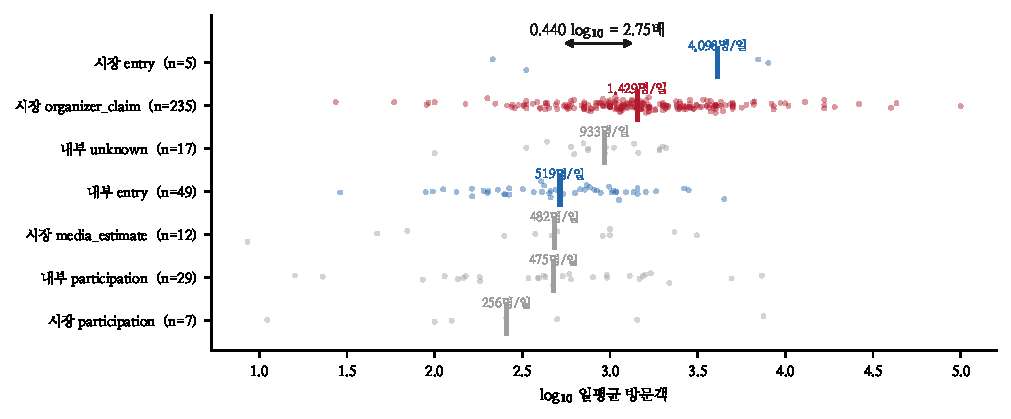
\includegraphics[width=\linewidth]{figs/unit_gap.pdf}
\caption{집계 기준별 log$_{10}$ 일평균 방문객. 점 하나가 팝업 하나이고, 세로 막대는
집단 중앙값이다. 붉은색은 주최자 발표, 푸른색은 게이트 계수, 회색은 그 외.
표본 5건 이상인 기준만 표시했다. 두 중앙값이 2.75배 벌어져 있다.}
\label{fig:gap}
\end{figure*}

그림~\ref{fig:gap}에서 가장 큰 두 집단이 양 끝에 있다. 주최자 발표는 하루 1{,}429명,
게이트 계수는 하루 519명이 중앙값이다.

\claimx{주최자 발표와 게이트 계수는 서로 다른 물리량이다. 격차는
$0.440\,\text{log}_{10}$, 즉 2.75배이며, 집계 기준이 타깃 분산의 23.3\%($\eta^2$)를 설명한다.}
{두 기준의 표본이 서로 다른 종류의 행사에 치우쳐 있다면 --- 예컨대 주최자가 발표하는 팝업이
애초에 더 큰 행사라면 --- 이 격차는 측정 차이가 아니라 선택 편향이다. 장소 등급과 IP 규모를
통제한 뒤에도 격차가 남는지 확인해야 한다.}

\section{같은 행사를 두 번 재기}

집단 수준의 격차만으로는 측정 차이와 수요 차이를 구분할 수 없다. 같은 행사를 두 방식으로
잰 사례가 필요하다. 내부 레코드와 시장 레코드를 브랜드·기간·장소로 대조해 5쌍을 찾았다.

이 중 3쌍은 두 값이 \emph{정확히} 일치했다. 이는 독립적인 두 측정이 아니라,
내부 라벨이 보도자료에서 옮겨 적힌 것이다. 우리 "내부" 라벨의 일부가 실은 주최자 발표라는
뜻이며, 그 자체로 별개의 오염이다.

독립적인 2쌍은 표~\ref{tab:pairs}와 같다.

\begin{table}[t]\centering\tsize
\caption{같은 행사의 두 측정. RXPU2515는 이마트 쓱데이 연계 팝업으로,
내부 게이트 계수와 주최 측 발표가 6.9배 차이 난다.}
\label{tab:pairs}
\begin{tabular}{llr}
\toprule
레코드 & 측정 방식 & 값 \\
\midrule
\multirow{2}{*}{RXPU2515} & 게이트 계수 & 2{,}305 \\
 & 주최자 발표 & 15{,}854 \\
\multicolumn{2}{r}{\itshape 격차} & \itshape 6.88배 \\
\midrule
\multirow{2}{*}{RTPU2440} & 내부 집계 & 9{,}000 \\
 & 언론 추정 & 7{,}500 \\
\multicolumn{2}{r}{\itshape 격차} & \itshape 0.83배 \\
\bottomrule
\end{tabular}
\end{table}

\claimx{같은 행사를 게이트로 세면 2{,}305명, 주최자가 발표하면 15{,}854명이다.
집단 수준 격차 2.75배는 개별 사례에서 6.9배까지 벌어진다.}
{독립 대조가 2쌍뿐이고, 그중 결정적인 것은 1쌍이다. 이 사례가 예외적으로 극단적일 수 있다.
내부·시장 중복 사례를 전수 탐색해 격차의 분포를 확인해야 한다.}

\section{전사 오류는 이보다 훨씬 작다}

라벨이 틀리는 또 다른 경로가 있다. 문서 안에서 총계와 일별 표가 어긋나는 경우다.
원문 재발굴로 4건을 규명했다(표~\ref{tab:transcription}).

\begin{table}[t]\centering\tsize
\caption{문서 내부 전사 오류. 전부 총계 쪽이 부분합이었고, 일별 표가 옳았다.}
\label{tab:transcription}
\begin{tabular}{p{1.55cm}p{3.3cm}r}
\toprule
레코드 & 원인과 확인 방법 & 격차 \\
\midrule
RTPU2582 & 총계가 마지막 2일 절단. 리플렛 재고(입고 4{,}000 $-$ 전시 150 $-$ 잔여 652)로 검증 & 1.13배 \\
RIPU2520 & 문서 내부 불일치 736명. 대조할 정산·POS 부재로 미해소 & 1.10배 \\
RTPU2454 & 인쇄 총계가 12/19 행 누락. 같은 표의 다른 합계는 전부 정확 & 1.09배 \\
RIPU2602 & 총계가 4/14 하루 누락. 일별 매출 합이 세금계산서와 원 단위 일치 & 1.08배 \\
\bottomrule
\end{tabular}
\end{table}

중앙값 $0.040\,\text{log}_{10}$ = 1.10배다. 집계 기준 격차의 1/7 수준이다.

\begin{figure}[t]\centering
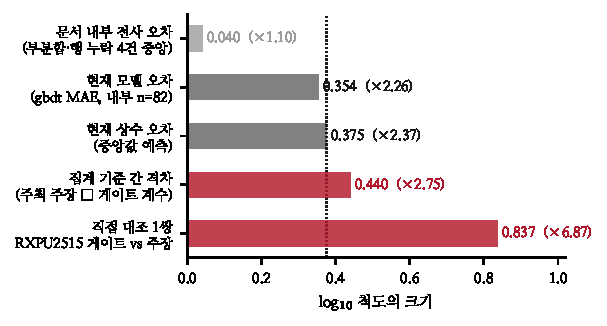
\includegraphics[width=\linewidth]{figs/error_scales.pdf}
\caption{오차 척도의 비교. 점선은 현재 상수 예측 오차. 전사 오류는 모델 오차보다 한참
작고, 집계 기준 격차는 모델 오차보다 크다.}
\label{fig:scales}
\end{figure}

\claimx{우리가 다뤄 온 오차는 전사 실수가 아니라 정의 혼재다.
전사 오류 1.10배 $\ll$ 모델 오차 2.37배 $<$ 기준 격차 2.75배.}
{전사 오류 4건은 재발굴로 \emph{발견된} 것만 세었다. 발견되지 않은 오류가 체계적으로
크다면 이 순서가 바뀔 수 있다. 무작위 표본을 뽑아 전수 대조해야 한다.}

\section{함의}

그림~\ref{fig:scales}의 순서가 이 연구의 결론이다. \textbf{현재 모델 오차가 집계 기준
격차보다 작다.} 자와 눈금이 2.75배 어긋난 상태에서 소수점을 다투고 있었던 셈이다.

이를 직접 보이기 위해, 피처를 하나도 쓰지 않고 집계 기준별로 중앙값만 예측해 보았다.

\begin{figure}[t]\centering
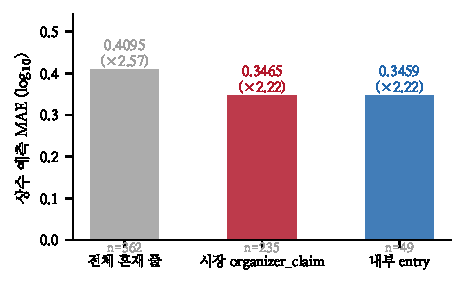
\includegraphics[width=\linewidth]{figs/pool_purity.pdf}
\caption{풀을 동질화하면 상수 예측 오차가 줄어든다. 모델을 쓰지 않고 정의만 정리한 결과다.}
\label{fig:purity}
\end{figure}

전체 혼재 풀에서 MAE 0.4095였던 것이 기준별로 나누면 0.346으로 떨어진다(15.5\% 개선).
참고로 132개 피처를 붙인 능선회귀의 혼재 풀 개선폭은 9.2\%였다.

\claimx{정의를 정리하는 것이 피처를 붙이는 것보다 이 규모에서 효과가 크다.
피처 0개 + 기준 층화 = 15.5\% 개선, 피처 132개 = 9.2\% 개선.}
{기준별 상수 예측은 예측 대상의 집계 기준을 \emph{안다}고 가정한다. 실제 예측 시점에
그 라벨이 어떤 기준으로 집계될지 모른다면 이 개선은 실현되지 않는다. 다만 우리 용도에서는
예측 대상의 집계 방식을 우리가 정하므로 가정이 성립한다.}

\section{한계와 다음 단계}

이 연구는 진단이며 처방이 아니다. 확정된 것과 열린 것을 구분해 둔다.

\paragraph{확정}
라벨 풀은 최소 두 개의 물리량을 담고 있고 격차는 2.75배다. 전사 오류는 그 1/7이므로
데이터 위생 작업의 한계 효용은 여기까지다. 혼재 풀에서 측정한 모델 성능은 해석할 수 없다.

\paragraph{열린 것}
직접 대조 쌍이 2개뿐이라 격차의 분포를 모른다. 기준 격차 중 선택 편향으로 설명되는 부분을
통제하지 않았다. 무엇보다, 동질 풀 내부의 \emph{환원 불가능한} 측정 오차 --- 같은 기준으로
두 번 재도 남는 차이 --- 는 아직 재지 못했다. 이를 재려면 같은 기준의 반복 측정이 필요한데
현재 0건이다.

\paragraph{다음 단계}
(1) 내부·시장 중복 사례를 전수 탐색해 격차 분포를 얻는다.
(2) 시장 라벨 263건의 집계 기준을 원문에서 재판정한다. 현재 235건이
\texttt{organizer\_claim}으로 뭉뚱그려져 있는데, 그 안에 게이트 계수를 인용한 보도가
섞여 있을 수 있다. 이 작업이 동질 풀의 크기를 결정한다.
(3) 동질 풀만으로 학습 파이프라인을 재구성하고 그 위에서 피처 절제를 다시 검정한다.

\vspace{0.7em}
\hrule
\vspace{0.4em}
{\footnotesize\color{black!60}
모든 수치는 저장소 상태 2026년 7월 28일 기준이며, 그림 생성 코드가 데이터에서 직접
계산한다. 라벨이 갱신되면 그림과 표도 함께 바뀐다. 재현: \texttt{python3 paper/figs.py}.}

\end{document}
